\chapter{Webographie}
\begin{itemize}
\item EPITA \\
  \texttt{www.epita.fr}
\item INRIA \\
  \texttt{www.inria.fr}
\item LRDE \\
  \texttt{www.lrde.epita.fr}
\item Langage Ocaml \\
  \texttt{www.caml.inria.fr}
\item PPS \\
  \texttt{www.pps.univ-paris-diderot.fr}
\item Projet Coq \\
  \texttt{www.coq.inria.fr}
\item \pir \\
  \texttt{http://www.pps.univ-paris-diderot.fr/pi.r2/}
\end{itemize}

\chapter{Annexes}
  \section{Sommaire des Annexes}
  \minitoc
  \section{Documentation sur l'entreprise}
  \subsection{Les membres du conseil d'administration de l'INRIA}
  Le tableau suivant présente les membres actuels (15 janvier 2013) du conseil
  d'administration de l'INRIA: \par
      \begin{tabular}{|l|p{8cm}|}
    \multicolumn{2}{l}{\textbf{Président} : Michel Cosnard, président directeur général de
    l'INRIA} \\
    \multicolumn{2}{l}{\textbf{Membre de droit} : Alain Fuchs, président directeur général
    du CNRS} \\
        \multicolumn{2}{l}{\textbf{Représentants de l'état} :} \\
        \hline
        Marc Bellœil &
        Chargé de mission, département Organismes spécialisés, DGRI (Recherche) \\
        \hline
        Fabien Terraillot & Chef du bureau du logiciel, DGCIS (Industrie) \\
        François Pouget & Chef du bureau 3 (MIRES), direction du Budget (Budget) \\
        \hline
        Éric Grégoire &
        Conseiller scientifique de formation, DGESIP (Enseignement supérieur) \\
        \hline
        Christine Marteau & Responsable du pôle Télécommunications, DGA (Défense) \\
        \hline
        Pascal le Deuff &
        Sous-directeur des échanges scientifiques et de la recherche (Affaires étrangères) \\
        \hline
        Cécile Dubarry &
        Chef du service des technologies de l’information et de la communication, DGCIS (Télécommunications) \\
        \hline
        \multicolumn{2}{l}{\textbf{Membres nommés} :}\\
        \hline
        Jean-Luc Beylat & Président d’Alcatel-Lucent Bell Labs France \\
        \hline
        Bernard Jarry-Lacombe & Secrétaire national CFDT cadres \\
        \hline
        Marie-Noëlle Jégo-Laveissière & Directrice recherche et développement,
        Orange Labs \\
        \hline
        Gilles Le Calvez & Directeur R\&D du Groupe Valeo \\
        \hline
        Brigitte Plateau & Administrateur général INP Grenoble \\
        \hline
        Luc Pabœuf & Président du CESR d’Aquitaine \\
        \hline
        Laure Reinhart & Directrice générale déléguée, OSEO et OSEO Innovation \\
        \hline
        Gérard Roucairol & Président de l’association Ter@tec \\
        \hline
        \multicolumn{2}{l}{\textbf{Membres élus : Représentants des personnels scientifiques}} \\
        \hline
        Serge Steer & Directeur de recherche, Inria Paris-Rocquencourt \\
        \hline
        Jocelyne Erhel & Directrice de recherche, Inria Rennes - Bretagne Atlantique \\
        \hline
        Lisette Calderan & Ingénieur de recherche, Inria Siège \\
        \hline
        Laurent Pierron & Ingénieur de recherche, Inria Nancy - Grand Est \\
        \hline
        \multicolumn{2}{l}{\textbf{Voix consultatives :}} \\
        \hline
        Malika Moha & Contrôleur général \\
        \hline
        Marie-Laure Inisan-Ehret & Agent comptable \\
        \hline
        Chris Hankin & Président du conseil scientifique \\
        \hline
        Antoine Petit & Directeur général adjoint \\
        \hline
    \end{tabular}
    \clearpage{}
  \section{Documentation sur le matériel/les logiciels}
  \subsection{Table de traduction des symboles dans Coqdoc}

  \begin{center}
    \begin{tabular}{|l|l|}
      \hline
      Le symbole & est traduit en                   \\ \hline
      \texttt{->}              & $\rightarrow$      \\ \hline
      \texttt{<-}              & $\leftarrow$       \\ \hline
      \texttt{*}               & $\times$           \\ \hline
      \texttt{<=}              & $\leq$             \\ \hline
      \texttt{>=}              & $\geq$             \\ \hline
      \texttt{=>}              & $\Rightarrow$      \\ \hline
      \texttt{<>}              & $\neq$             \\ \hline
      \texttt{<->}             & $\leftrightarrow$  \\ \hline
      \texttt{|-}              & $\vdash$           \\ \hline
      \texttt{\textbackslash/} & $\land$            \\ \hline
      \texttt{/\textbackslash} & $\lor$             \\ \hline
      \texttt{\~}              & $\lnot$            \\ \hline
    \end{tabular}
    \label{trad.coqdoc}
  \end{center}
  \clearpage{}
  \section{Résultats bruts}
  \label{results}
  Les images qui suivent donnent un exemple de documents générés par Coqdoc.
  \begin{figure}
  \fbox{
  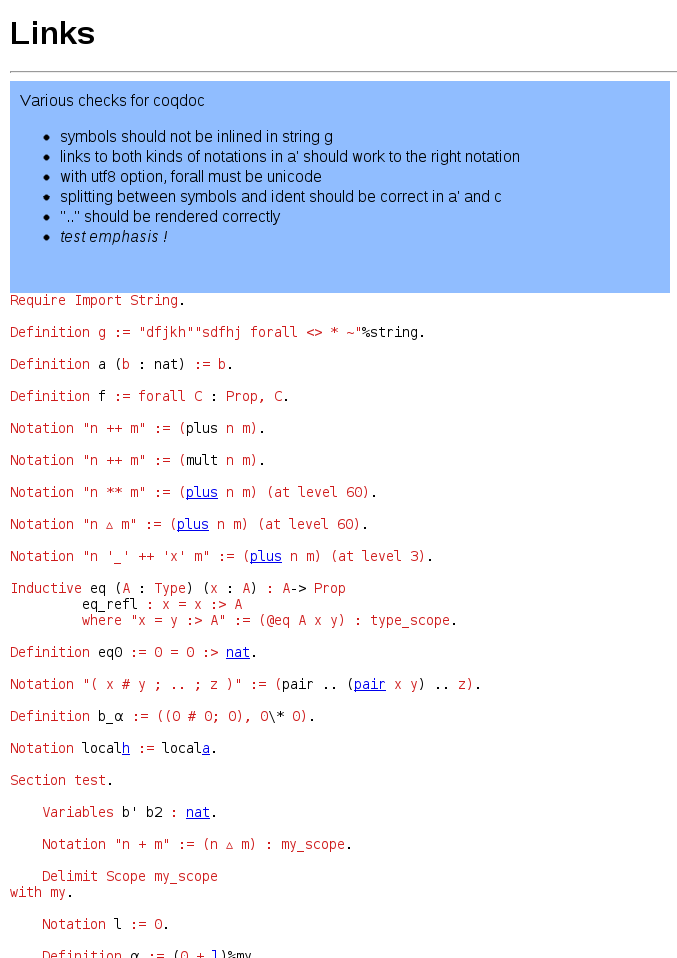
\includegraphics[scale=0.7]{../data/html.png}}
  \caption{Exemple de rendu en HTML}
  \end{figure}
  \clearpage
  \begin{figure}
  \fbox{
  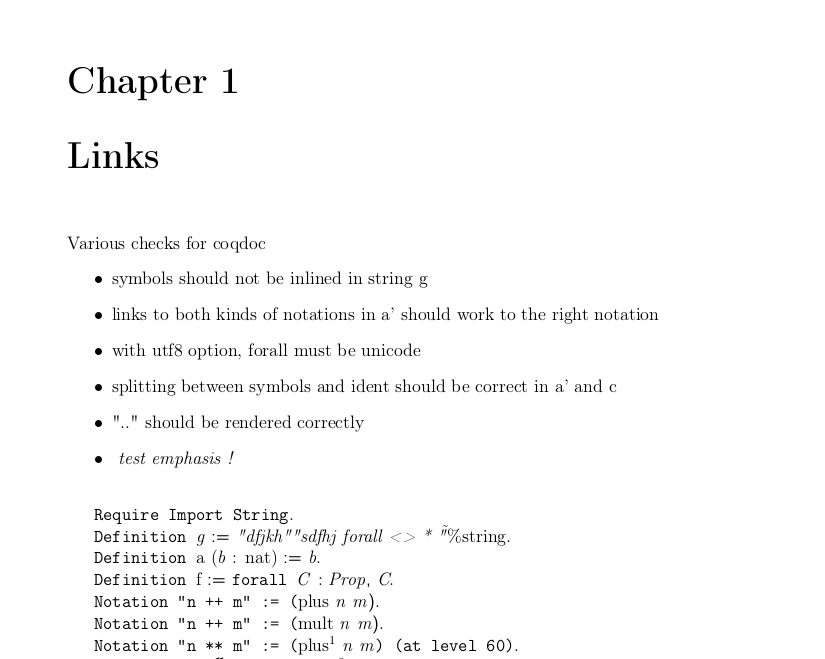
\includegraphics[scale=0.7]{../data/pdf.png}}
  \caption{Exemple de rendu en LateX}
  \end{figure}
  \clearpage
  %% FIXME: faire des copies d'écran pour le HTML et inclure le pdf
